% Created 2023-12-08 Fri 17:08
% Intended LaTeX compiler: pdflatex
\documentclass[11pt]{article}
\usepackage[utf8]{inputenc}
\usepackage[T1]{fontenc}
\usepackage{graphicx}
\usepackage{longtable}
\usepackage{wrapfig}
\usepackage{rotating}
\usepackage[normalem]{ulem}
\usepackage{amsmath}
\usepackage{amssymb}
\usepackage{capt-of}
\usepackage{hyperref}
\usepackage{minted}
\usepackage{minted}
\author{Jonathan Ulmer}
\date{\today}
\title{Bsc Thesis}
\hypersetup{
 pdfauthor={Jonathan Ulmer},
 pdftitle={Bsc Thesis},
 pdfkeywords={},
 pdfsubject={},
 pdfcreator={Emacs 28.3 (Org mode 9.7)}, 
 pdflang={English}}
\usepackage{biblatex}
\addbibresource{~/org/resources/bibliography/refs.bib}
\begin{document}

\maketitle
\tableofcontents

\section{Cahn Hillard Equation Overview}
\label{sec:org8a3c2ff}
Partial Differential Equation (PDE) solving the state of a 2 Phase Fluid\autocite{Wu_2022}. The form of the Cahn Hillard Equation used for the remainder of this thesis is:
\begin{align}
\phi _t(x,t) &=  \Delta  \mu \\
\mu &= - \varepsilon^2 \Delta \phi   + W'(\phi)
\end{align}
where \(\phi\) is the so called phase field. Demarking the different states of the fluids through an Interval \(I=[-1,1]\) and where \(\partial I = \{-1,1\}\)  represents full state of one fluid. \(\varepsilon > 0\) is  a positive constant

, and \(\mu\) is the chemical potential\autocite{Wu_2022}. While the Cahn Hillard exist in a more general form taking the fluids mobility \(M(\Phi)\) into account, we will assume \(M(\Phi) = 1\), simplifying the CH-Equations used in\autocite{Wu_2022}\autocite{SHIN20117441} to what is stated above.


The Advantages of the Cahn Hillard Approach as compared to traditional fluid dynamics solvers are for example: ``explicit tracking of the interface'' \autocite{Wu_2022}, as well as ``evolution of complex geometries and topological changes [\ldots{}] in a natural way'' \autocite{Wu_2022}
\subsection{{\bfseries\sffamily TODO} Derivation from paper}
\label{sec:org52b80ab}
\subsubsection{Free energy}
\label{sec:org8bd12f1}
The Cahn Hillard Equations can be motivated Using a \textbf{Ginzburg Landau} type free energy equation:
\begin{align*}
E^{\text{bulk}}  = \int_{  \Omega}  \frac{\varepsilon^2}{2} |\nabla \phi |^2 + F(\phi) \,dx
\end{align*}
where ``\(F(\phi)\)  denotes the (Helmholtz) free energy density of mixing.''`` \autocite{Wu_2022} and will be approximated in further calculations as \(F(\phi) = \frac{(1-\phi ^2)^2}{4}\) as used in\autocite{SHIN20117441}

The chemical potential then follows as derivative of Energy in respect to time.
\begin{align*}
 \mu &= \frac{\delta E_{bulk}(\phi)}{\delta \phi } = -\varepsilon^2 \Delta \phi  + W'(\phi)
\end{align*}
\subsubsection{Derivation by mass balance}
\label{sec:orgaadf4c8}
The Cahn Hillard equation then can be motivated as follows:
consider
\begin{equation}
    \partial_t \phi + \nabla J  = 0
\end{equation}
where   \textbf{J} is mass flux. eq1 then states that the change in mass balances the change of the phasefield.
using the no-flux boundry conditions:
\begin{align}
J \cdot n &= 0  & \partial\Omega &\times (0,T)\\
\partial_n\phi  &= 0  & \partial\Omega &\times (0,T)
\end{align}
conservation of mass follows see\autocite{Wu_2022}.

using:
\begin{align}
J &= - \nabla \mu
\end{align}
which conceptionally sets mass flux to equalize the  the potential energy gradient, leads to the formulation of the CH equations as stated above. additionally the boundry conditions evaluate to:
\begin{align*}
 - \nabla \mu &= 0 \\
\partial_n \phi  = 0
\end{align*}
ie no flow leaves and potential on the border doesn't change.
then for \(\phi\) then follows:
\begin{align*}
\frac{d}{dt}E^{bulk}(\phi(t)) &= \int_{\Omega} (\varepsilon^2 \nabla \phi \cdot \nabla \partial_t \phi + W'(\phi) \partial_t \phi) \ d x  \\
&= - \int_{  \Omega } |\nabla \mu|^2 \ d x, & \forall t \in  (0,T)
\end{align*}
hence the Free Energy is decreasing in time.
\section{Baseline Multigrid solver:}
\label{sec:org46fde8d}
As baseline for further experiments a multi grid method based on finite differences by\autocite{SHIN20117441}. is used.
\subsection{Discretization:\hfill{}\textsc{ATTACH}}
\label{sec:org6f425c3}
it discretizes the phasefield and potential energy \(\phi, \mu\) into a grid wise functions \(\phi_{ij}, \mu_{ij}\) and defines the partial derivatives \(D_xf_{ij}, \  D_yf_{ij}\) using the differential quotients:
\begin{align*}
D_xf_{i+\frac{1}{2} j} &= \frac{f_{i+1j} - f_{ij}}{h} & D_yf_{ij+\frac{1}{2}} &= \frac{f_{ij+1} - f_{ij}}{h}
\end{align*}
for \(\nabla f , \Delta f\) then follows:
\begin{align*}
\nabla_d f_{ij} &= (D_x f_{i+1j} , \ D_y f_{ij+1}) \\
 \Delta_d f_{ij} &= \frac{D_x f_{i+\frac{1}{2}j} -  D_x f_{i-\frac{1}{2}j} + D_y f_{ij+\frac{1}{2}} - D_y f_{ij-\frac{1}{2}}}{h} = \nabla_d \cdot  \nabla_d f_{ij}
\end{align*}
the authors further adapt the discretized phasefield by the characteristic function of the domain \(\Omega\):
\begin{align*}
G(x,y) &=
\begin{cases}
1 & (x,y) \in  \Omega \\
0 & (x,y) \not\in  \Omega
\end{cases}
\end{align*}
To account for boundry conditions and arbitrary shaped domains.
The authors \autocite{SHIN20117441} then define the discrete CH Equation adapted for Domain, as:
\begin{align*}
\frac{\phi_{i+1j} - \phi_{ij}}{\Delta t}  &=  \nabla _d \cdot (G_{ij} \nabla_d \mu_{ij}^{n+1} )  \\
 \mu_{ij}^{n+1} &= 2\phi_{ij}^{n+1} - \varepsilon^2  \nabla_d \cdot  (G_{ij} \nabla _d \phi_{ij}^{n+1} ) + W'(\phi_{ij}^n) - 2\phi _{ij}^n
\end{align*}
and derive the iteration operator \(L(\phi^{n+1} , \mu^{n+\frac{1}{2}}) = (\zeta^n ,\psi^n)\)
\begin{align*}
L
\begin{pmatrix}
\phi^{n+1} \\
\mu^{n+\frac{1}{2}}
\end{pmatrix}
&=
\begin{pmatrix}
\frac{\phi^{n+1}}{\Delta t} - \nabla _d \cdot  ( G_{ij} \nabla _d \mu^{n+\frac{1}{2}} ) \\
\varepsilon^2 \nabla _d \cdot  (G_{ij} \nabla_d \phi_{ij}^{n+1}) - 2\phi_{ij}^{n+1} + \mu_{ij}^{n+\frac{1}{2}}
\end{pmatrix}
\end{align*}
initialized as
\((\zeta^n, \psi^n) =
\left(\begin{smallmatrix}
\frac{\phi_{ij}^{n+1}}{\Delta t}\\
W'(\phi_{ij}^n) - 2\phi_{ij}^n
\end{smallmatrix}
\right)\)
the algorithm is then defined as:

wherein SMOOTH consists of point-wise Gauß Seidel Relaxation , by solving \emph{L} for \(\overline{\phi} ,\overline{\mu}\) with the initial guess for \(\zeta^n , \psi^n\).
\subsection{adaptations to the simplified problem}
\label{sec:orgeeaf564}
even tough this work uses rectangular domains, the adaptation of the algorithm is simplified by the domain indicator function, as well as 0 padding, in order to correctly include the boundry conditions of the CH equation.
therefore the internal representation of the adapted algorithm considers phasefield and potential field \(\phi , \mu\) as 2D arrays of shape \((N_X + 2 , N_y + 2)\) in order to accommodate padding. Where N\textsubscript{x} and N\textsubscript{y} are the number of steps in x- / y-Direction respectively.
Hence, we define the discrete domain function as:
\begin{align*}
G_{ij} &=
\begin{cases}
1 & (i,j) \in  [1,N_x+1] \times  [1,N_y+1] \\
0 & \text{else}
\end{cases}
\end{align*}
\subsection{tests\textsubscript{data}:}
\label{sec:org815283c}
\subsubsection{squares}
\label{sec:org9898bf1}
For testting and later training , a multitude o different phasefields where used. notably an assortment of rnadomly lpaced circles, squares, and arbetrary generated values
\begin{center}
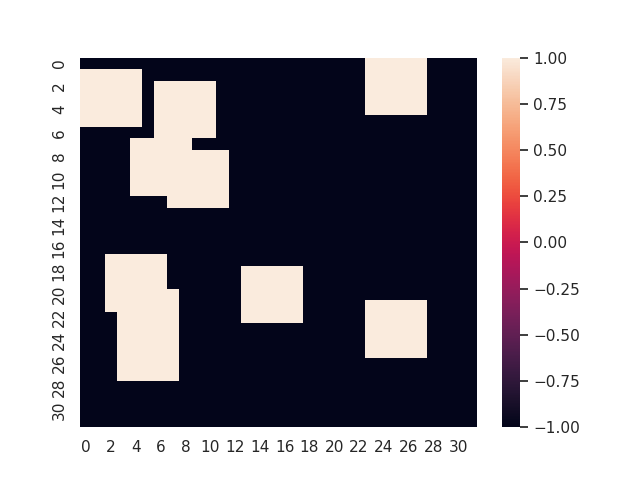
\includegraphics[width=.9\linewidth]{images/phase.png}
\end{center}



\begin{center}
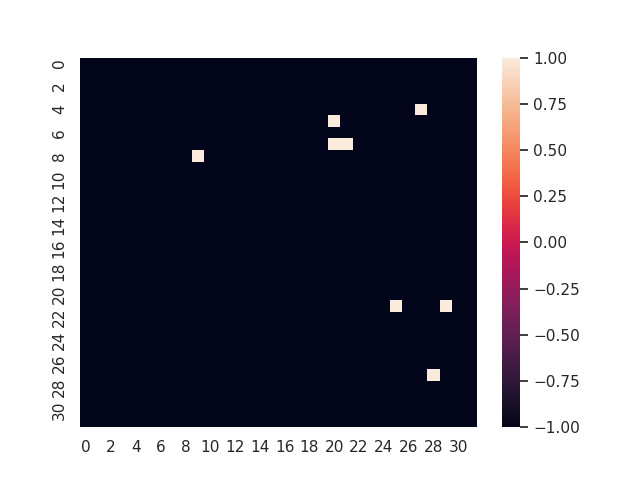
\includegraphics[width=.9\linewidth]{images/phase2.png}
\end{center}
\subsubsection{circles}
\label{sec:org4aa1f6d}
\subsection{Tests}
\label{sec:orgb49f240}

\begin{minted}[frame=lines,breaklines,linenos=true]{python}
test_phase = tu.k_spheres_phase(4,7)
solver = tu.setup_solver(test_phase)
solver.solve(4,10)
\end{minted}

\begin{minted}[frame=lines,breaklines,linenos=true]{python}
plt.figure()
sns.heatmap(solver.phase_small)
\end{minted}
\section{Relaxed Problem}
\label{sec:org24e0cd8}
In effort to decrease the order of complexity, the following relaxation to the classical CH Equation is proposed:
\begin{align*}
\partial_t \phi  &= \Delta \mu \\
\mu &= \varepsilon ^2(c^\alpha - \phi^\alpha) + W'(\phi)
\end{align*}
where \(c\) is the solution of the following elliptical PDE
\begin{align*}
- \Delta c^\alpha  + \alpha c^a &= \alpha \phi ^\alpha
\end{align*}
\subsection{{\bfseries\sffamily TODO} relaxed operators:}
\label{sec:org8087e9a}
\subsubsection{L Relaxed}
\label{sec:org93b82d1}
\begin{align*}
L
\begin{pmatrix}
\phi ^{n+1} \\
\mu^{n+1}
\end{pmatrix}
&=
\begin{pmatrix}
\frac{\phi^{n+1,m}_{ij}}{\Delta t} - \nabla _d \cdot (G_{ji} \nabla _d \mu^{n + \frac{1}{2},m}_{ji}) \\
\varepsilon ^2 (c^\alpha - (\phi^{n+1,m}_{ij})^\alpha) - 2\phi ^{n+1,m}_{ij} -\mu^{n + \frac{1}{2},m}_{ji}
\end{pmatrix}
\end{align*}
\subsubsection{SMOOTH}
\label{sec:org6e6768b}

\begin{align*}
SMOOTH( \phi^{n+1,m}_{ij}, \mu^{n + \frac{1}{2},m}_{ji}, L_h , \zeta ^n , \psi ^n )
\end{align*}
\begin{align*}
\overline{\mu}^{n + \frac{1}{2},m}_{ji}
&=
  \frac{\phi ^{n+1,m}_{ij}}{\Delta t} - \zeta^n_{ij} \\
&- \frac{1}{h^2}(G_{i+\frac{1}{2}j} \mu^{n + \frac{1}{2},m}_{i+1j} +  G_{i-1j} \mu^{n + \frac{1}{2},m}_{i-1j} + G_{ij+1}  \mu^{n + \frac{1}{2},m}_{ij+1} + G_{ij-1} \mu^{n + \frac{1}{2},m}_{ij-1}) \\
&\cdot  (G_{i+1j} + G_{i-1j} + G_{ij+1} + G_{ij-1})^{-1} \\
 \varepsilon ^2 (\overline{\phi} ^{n+1,m}_{ij})^\alpha + 2 \phi ^{n+1,m}_{ij} &= \varepsilon ^2 c^\alpha  -\mu^{n + \frac{1}{2},m}_{ji}  - \psi_{ij}
\end{align*}
\begin{enumerate}
\item Proposal
\label{sec:org644b61b}
design newton method to solve second equation (in conjunction with the first one) hopefully solving is faster than the original multiple SMOOTH Iterations.
 The iteration is to solve for \(\phi ^{n+1,m}_{ij}\) as free variable. Therefore it follows for \(F(x)\)

\begin{align*}
F(x)  &= \varepsilon ^2 x^\alpha + 2x - \varepsilon^2 c^\alpha  + y + \psi_{ij} \\
y &= \frac{x}{\Delta t} - \zeta^n_{ij} \\
&- \frac{1}{h^2}(G_{i+\frac{1}{2}j} \mu^{n + \frac{1}{2},m}_{i+1j} +  G_{i-1j} \mu^{n + \frac{1}{2},m}_{i-1j} + G_{ij+1}  \mu^{n + \frac{1}{2},m}_{ij+1} + G_{ij-1} \mu^{n + \frac{1}{2},m}_{ij-1}) \\
&\cdot  (G_{i+1j} + G_{i-1j} + G_{ij+1} + G_{ij-1})^{-1} \\
\end{align*}
And the derivative for the iteration is
\begin{align*}
\frac{d}{dx} F(x)&= \alpha \varepsilon^2 x^{\alpha-1} + 2 + \frac{d}{dx} y  \\
\frac{d}{dx} y  &= \frac{1}{\Delta t}
\end{align*}
\end{enumerate}
\subsection{Elliptical PDE:}
\label{sec:org2f4ef1c}
on order to solve the relaxed CH Equation the following PDE as to be solved in Each additional time step:
or in terms of the characteristic function:
\begin{align*}
- \nabla \cdot  (G \nabla c^\alpha) + \alpha c^\alpha  = \alpha \phi ^\alpha
\end{align*}
\subsubsection{Discretization}
\label{sec:org12de1ac}
Discretization of the PDE
\begin{align*}
- \nabla_d \cdot  (G_{ij} \nabla_d c_{ij}^\alpha) + \alpha  c_{ij}^\alpha &= \alpha \phi_{ij}^\alpha \\
- (\frac{1}{h}(G_{i+\frac{1}{2}j} \nabla c^\alpha_{i+\frac{1}{2}j} + G_{ij+\frac{1}{2}} \nabla c^\alpha_{ij+\frac{1}{2}}) &  \\
- (G_{i-\frac{1}{2}j} \nabla c^\alpha_{i-\frac{1}{2}j} + G_{ij-\frac{1}{2}} \nabla c^\alpha_{ij-\frac{1}{2}})) + \alpha  c_{ij}^\alpha   &= \alpha  \phi_{ij}^\alpha \\
\frac{1}{h^2} ( G_{i+\frac{1}{2}j}(c_{i+1j}^\alpha - c_{ij}^\alpha) & \\
+G_{ij+\frac{1}{2}}(c_{ij+1}^\alpha - c_{ij}^\alpha) &\\
+G_{i-\frac{1}{2}j}(c_{i-1j}^\alpha - c_{ij}^\alpha)&\\
+G_{ij-\frac{1}{2}}(c_{ij-1}^\alpha - c_{ij}^\alpha))&=\alpha  \phi_{ij}^\alpha \\
\end{align*}
\section{References}
\label{sec:orgfef094c}
\printbibliography
\end{document}